\documentclass[pdflatex,sn-mathphys-num,iicol]{sn-jnl}

\usepackage[T1]{fontenc}
\usepackage{amsmath,amssymb}
\usepackage{float}
\floatstyle{ruled}
\newfloat{algorithm}{tbp}{loa}
\floatname{algorithm}{Algorithm}
\usepackage{algpseudocode}
\usepackage{booktabs}
\usepackage{array}
\usepackage{graphicx}
\usepackage{tikz}
\usepackage{pgfplots}
\pgfplotsset{compat=1.17}
\usetikzlibrary{arrows.meta,calc,positioning}
\hypersetup{hypertexnames=false}
\newcommand{\ci}[3]{\begin{tabular}[c]{@{}c@{}}$#1$\\{}[$#2$, $#3$]\end{tabular}}
\newcommand{\cib}[3]{{\boldmath\ci{#1}{#2}{#3}}}
\newcommand{\cit}[3]{\begin{tabular}[t]{@{}c@{}}$#1$\\{}[$#2$, $#3$]\end{tabular}}
\newcommand{\cibt}[3]{{\boldmath\cit{#1}{#2}{#3}}}
\newcommand{\scl}{SCL}
\newcommand{\aob}{AOB}
\newcommand{\twol}[2]{\begin{tabular}[c]{@{}l@{}}#1\\#2\end{tabular}}

\raggedbottom
\setcounter{dbltopnumber}{2}

\begin{document}

\title[Self-Calibrating Control Layer for Multi-Object Trackers]{Training-Free Self-Calibrating Control Layer for Heterogeneous Multi-Object Trackers}

\author*[1]{\fnm{Ahmed Gouda} \sur{Ismail}}\email{a7medgouda1@gmail.com}
\author[1]{\fnm{Mohamed S.} \sur{Mohamed}}\email{mohamedms@mtc.edu.eg}
\author[2]{\fnm{Tarek Ahmed} \sur{Mahmoud}}\email{tarek.mohamed@eui.edu.eg}

\affil*[1]{\orgdiv{Computer Engineering and Artificial Intelligence Department}, \orgname{Military Technical College}, \orgaddress{\city{Cairo}, \country{Egypt}}}
\affil[2]{\orgdiv{Computer Engineering Department}, \orgname{Egypt University of Informatics}, \orgaddress{\city{Cairo}, \country{Egypt}}}

\abstract{Multi-object tracking pipelines are often built from a detector and a tracker developed separately. When the detector is replaced, retrained, or quantized for embedded hardware, its confidence scale changes, while the tracker keeps thresholds tuned for another detector. This paper presents \scl{}, a training-free self-calibrating control layer between a frozen detector and a frozen tracker. It calibrates itself online with nested Otsu thresholds on the detector logits of recent frames and decides whether the score stream is clean or noisy. On clean streams it keeps the tracker's operating point. On noisy streams it selects the candidates that reach the tracker, remaps their scores, and sets the tracker's thresholds. It also gives a continuation stage to trackers that lack one. It needs no labels and uses no future frames. One frozen configuration was evaluated on nine published trackers, four detection sources, and three datasets with paired bootstrap intervals. It raised the higher order tracking accuracy (HOTA) of OC-SORT and of the external PD-SORT by 0.61 points, with intervals above zero. When the detector scores were halved, it restored two trackers from 0 to about 66 HOTA. With a noisy RT-DETR-L detector, it raised the multi-object tracking accuracy (MOTA) of ByteTrack and BoT-SORT by 6.0 and 7.9 points. On five trackers with a low-score stage and well-matched detections, HOTA changed by at most 0.06 points. \scl{} takes 2.95 ms per frame on a four-core CPU without a GPU, so it adds very little latency and is suitable for real-time use.}

\keywords{Multi-object tracking, Tracking by detection, Detector confidence calibration, Online adaptation, Otsu thresholding, Real-time image processing}

\maketitle

\section{Introduction}\label{sec:intro}

Multi-object tracking (MOT) finds every object of interest in a video and
keeps the same identity for each object over time. It is a core part of
surveillance, driving, and airborne systems
\cite{zhu2022visdrone,wu2022uavsurvey,lu2024uavdetection}, and many of these systems
must produce results with low delay. Most practical trackers follow the
tracking-by-detection design. A detector scores candidate boxes in each frame,
and the tracker links the boxes whose scores pass its thresholds into
trajectories \cite{bewley2016sort,zhang2022bytetrack,cao2023ocsort}.

In deployed systems the detector and the tracker are rarely developed
together. A detector is replaced by a faster model, retrained for a new
sensor, or quantized for embedded hardware. The tracker, however, keeps the
thresholds that its authors tuned for another detector. Detector confidence is
not calibrated across models and conditions \cite{kuppers2020detcalib}, so the
new detector usually has a different score scale, and nothing in the pipeline
notices the change.

The effect can be large. In the experiments of this paper, halving the scores
of a published detector drives two well-known trackers to 0 higher order
tracking accuracy (HOTA) \cite{luiten2021hota}, because no detection reaches
their fixed thresholds (Sect.~\ref{sec:shift}). Retuning
every tracker for every detector needs labelled data from the deployment
domain, which an operational system usually does not have.

Existing methods only partly address this problem. Adaptive-threshold
trackers adjust their own thresholds from the detections of each frame, but
each method is built into one specific tracker
\cite{ma2023adaptivebytetrack,shim2024adaptrack,act2026adaptive}. Confidence
calibration methods correct the detector scores, but they need labelled data
\cite{kuppers2020detcalib}. Adaptive inference methods learn or profile a
policy for one model \cite{han2022dynamic,jiang2018chameleon}. What is missing
is a training-free component that works outside the tracker, calibrates itself
from the detector's own score stream, and leaves the tracker unchanged when
the tracker already fits that stream.

This paper presents such a component: \scl{}, a self-calibrating control layer
between a frozen detector and a frozen tracker. It reads the stream of detector scores
and the operating point that the tracker declares, and it decides online
whether the tracker needs help. \scl{} is described in
Sect.~\ref{sec:method}, and Sect.~\ref{sec:development} explains how it was
developed from an earlier design that always intervened.

The main contributions are:
\begin{enumerate}
\item \scl{}, a training-free control layer that calibrates itself from the detector
      score stream and changes the tracker's input only when the stream is
      noisy (Sect.~\ref{sec:method}).
\item A host contract of four numbers that lets one frozen configuration work
      with single-stage, two-stage, coordinate-only, and two-view trackers
      without modifying them (Sect.~\ref{sec:contract}).
\item A development path from always-on banding (\aob{}), a prior design that
      always intervened, in which
      each step is compared with that baseline (Sect.~\ref{sec:development}).
\item An evaluation of one frozen configuration on nine published trackers,
      four detection sources, and three datasets, with development,
      predeclared, and post-freeze roles, paired bootstrap intervals, and a
      latency measurement on a CPU (Sects.~\ref{sec:setup}
      and~\ref{sec:results}).
\end{enumerate}

The rest of the paper is organized as follows. Section~\ref{sec:related}
reviews related work. Section~\ref{sec:method} describes \scl{}, and
Section~\ref{sec:development} explains how it was developed.
Section~\ref{sec:setup} gives the experimental setup,
Section~\ref{sec:results} the results, and Section~\ref{sec:discussion} a
discussion. Section~\ref{sec:conclusion} concludes the paper.

\section{Related Work}\label{sec:related}

\subsection{Tracking by detection}
SORT predicts each box with a Kalman filter and matches the predictions to new
detections by overlap with the Hungarian method \cite{bewley2016sort}.
StrongSORT and BoT-SORT add appearance features
\cite{du2023strongsort,aharon2022botsort}. ByteTrack
introduced a second association stage that uses low-confidence detections to
continue existing tracks \cite{zhang2022bytetrack}. This two-stage design was
kept by BoT-SORT \cite{aharon2022botsort}, SparseTrack \cite{liu2025sparsetrack},
BoostTrack \cite{stanojevic2024boosttrack}, and Hybrid-SORT
\cite{yang2024hybridsort}. OC-SORT \cite{cao2023ocsort}, Deep OC-SORT
\cite{maggiolino2023deepocsort}, and PD-SORT \cite{wang2025pdsort} use a single
confidence threshold. Recent designs learn association from box coordinates
(C-TWiX \cite{miah2025twix}), run parallel association paths (TOPICTrack
\cite{cao2025topictrack}), or associate two detection views (TrackTrack
\cite{shim2025tracktrack}). End-to-end trackers predict identities directly
\cite{zeng2022motr,gao2025motip}. All of these trackers read detector scores
through fixed thresholds that were tuned for one detector, usually YOLOX
\cite{ge2021yolox}. Nine of them are used in this paper as hosts and are kept
unchanged.

\subsection{Detector confidence and calibration}
Detectors of different families, such as YOLOX \cite{ge2021yolox}, YOLOv8
\cite{jocher2023yolov8}, YOLOv9 \cite{wang2024yolov9}, DETR
\cite{carion2020detr}, and RT-DETR
\cite{zhao2024rtdetr}, produce different score distributions. Their confidence
is not calibrated across models and conditions, and calibration methods for
object detection fit a mapping on labelled data \cite{kuppers2020detcalib}.
Otsu's method selects a threshold from a histogram without labels by
maximizing the separation between two classes \cite{otsu1979}. \scl{}
applies it to the detector logits of recent frames.

\subsection{Adaptive thresholds inside trackers}
Several trackers adapt their own confidence thresholds. Adaptive ByteTrack
derives the confidence threshold of ByteTrack from the detections of each
frame \cite{ma2023adaptivebytetrack}. AdapTrack adapts the thresholds of its
matching step \cite{shim2024adaptrack}. ACT sets the high and low thresholds
of each frame from the first quartile of the confidence scores and the number
of candidates \cite{act2026adaptive}. These methods are built into one tracker
and use statistics of the current frame. \scl{} differs in
four ways. Its statistics come from past frames. It decides for the whole
stream whether to intervene at all, and otherwise keeps the tracker's own
operating point. It acts through a declared host contract on several
published trackers without modifying them. It is evaluated as one frozen
policy under confidence shift and on external systems.

\subsection{Adaptive inference}
Dynamic neural networks adapt their computation to each input
\cite{han2022dynamic}, and Chameleon re-profiles the configuration of video
analytics pipelines over time \cite{jiang2018chameleon}. These methods learn or
profile a policy for each model. A controller that sets the detector operating
point from image cues is also tied to the detector it was calibrated with,
because a change of the detector's score scale leaves the image unchanged.
\scl{} reads the score stream instead and acts on the
tracker's input and thresholds. Table~\ref{tab:related} summarizes the
differences.

\begin{table}[t]
\caption{Adaptive methods closest to \scl{} (BT: ByteTrack).}
\label{tab:related}
\centering\footnotesize
\setlength{\tabcolsep}{3pt}
\begin{tabular}{@{}>{\raggedright\arraybackslash}p{17mm}>{\raggedright\arraybackslash}p{18mm}>{\raggedright\arraybackslash}p{15mm}>{\raggedright\arraybackslash}p{18mm}@{}}
\toprule
Method & Adapted & Statistics & Where\\
\midrule
Adapt.\ BT \cite{ma2023adaptivebytetrack} & confidence threshold & current frame & inside BT\\
AdapTrack \cite{shim2024adaptrack} & matching thresholds & current frame & inside the tracker\\
ACT \cite{act2026adaptive} & high and low thresholds & current frame & inside the tracker\\
K{\"u}ppers \cite{kuppers2020detcalib} & detector scores & labelled data & detector output\\
Chameleon \cite{jiang2018chameleon} & pipeline configuration & profiling & analytics pipeline\\
\scl{} (this paper) & candidates, scores, thresholds & past frames, no labels & between detector and tracker\\
\bottomrule
\end{tabular}
\end{table}

\section{Method}\label{sec:method}

\subsection{Problem setting}\label{sec:problem}
At frame $t$ a frozen detector emits candidates $D_t=\{(\mathbf{x}_i,s_i,c_i)\}$
with boxes $\mathbf{x}_i$, scores $s_i\in(0,1)$, and class labels $c_i$, down
to an emission floor. The layer works on the logit of each score,
\begin{equation}
z_i=\log\frac{s_i}{1-s_i}.
\label{eq:logit}
\end{equation}
A frozen tracker, called the host, declares a host contract
$h=(a,b,\ell,m_0)$. Here $a$ is the score threshold of its first association,
$b$ is the lowest score from which a new track can start, $\ell$ is the lowest
score that any of its association stages uses, and $m_0$ is its matching
tolerance (one minus its minimum overlap). A single-stage tracker has
$\ell=\min(a,b)$, and a two-stage tracker has $\ell<\min(a,b)$.

For every frame the layer outputs the set $K_t$ of candidates passed to the
tracker, the scores $\tilde{s}$ passed with them, and the thresholds
$(a_t,b_t)$ and tolerance $m_t$ that the tracker uses in that frame:
\begin{equation}
\left(K_t,\tilde{s},a_t,b_t,m_t\right)=
\mathcal{L}\left(Z_{<t},D_t,\mathcal{T}_{t-1},g_t;\,h\right).
\label{eq:layer}
\end{equation}
$Z_{<t}$ are the logits of earlier frames, $\mathcal{T}_{t-1}$ are the
tracks that the tracker reported for frame $t-1$, and $g_t$ is an optional
image-motion cue of frame $t$. The layer works online. Its statistics use only
frames before $t$, and the data of frame $t$ enter its state after the
decision. No future frame is used.

The layer has four requirements: it needs no training and no labelled
calibration data; one frozen configuration serves every tracker, detector, and
dataset; the output stays unchanged when the tracker's operating point already
fits the score stream; and its cost per frame is small next to the detector.

\subsection{Overview}
Figure~\ref{fig:arch} shows \scl{}. It has four parts: stream statistics, a
regime estimate, a candidate policy for each regime, and a continuation
rescue. The host contract enters the rescue and the thresholds passed to the
tracker. The detector and the tracker are not modified.

\begin{figure*}[t]
\centering
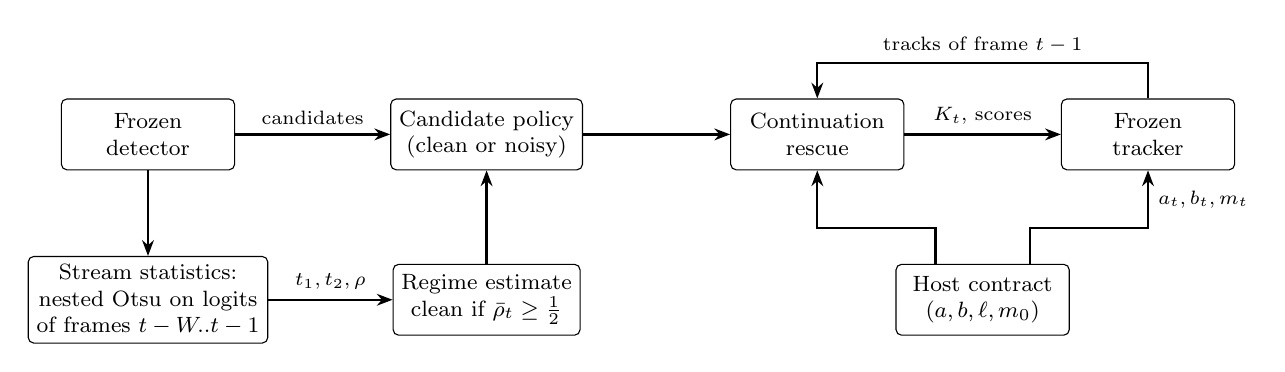
\begin{tikzpicture}[
  box/.style={draw, rounded corners=2pt, align=center, font=\footnotesize, minimum height=9mm, minimum width=22mm, inner sep=3pt},
  arr/.style={-{Stealth[length=2mm]}, thick}, lab/.style={font=\scriptsize}]
\node[box] (det) at (0,0) {Frozen\\detector};
\node[box] (pol) at (4.3,0) {Candidate policy\\(clean or noisy)};
\node[box] (res) at (8.5,0) {Continuation\\rescue};
\node[box] (trk) at (12.7,0) {Frozen\\tracker};
\node[box] (stat) at (0,-2.1) {Stream statistics:\\nested Otsu on logits\\of frames $t-W..t-1$};
\node[box] (reg) at (4.3,-2.1) {Regime estimate\\clean if $\bar\rho_t \ge \tfrac12$};
\node[box] (hc) at (10.6,-2.1) {Host contract\\$(a, b, \ell, m_0)$};
\draw[arr] (det) -- node[lab, above]{candidates} (pol);
\draw[arr] (pol) -- (res);
\draw[arr] (res) -- node[lab, above]{$K_t$, scores} (trk);
\draw[arr] (det) -- (stat);
\draw[arr] (stat) -- node[lab, above]{$t_1, t_2, \rho$} (reg);
\draw[arr] (reg) -- (pol);
\draw[arr] (hc.north) ++(-0.6,0) |- ++(0,0.45) -| (res.south);
\draw[arr] (hc.north) ++(0.6,0) |- ++(0,0.45) -| node[lab, pos=0.75, right]{$a_t, b_t, m_t$} (trk.south);
\draw[arr] (trk.north) -- ++(0,0.45) -| node[lab, pos=0.25, above]{tracks of frame $t-1$} (res.north);
\end{tikzpicture}
\caption{Self-calibrating control layer (\scl{}) between a frozen detector and a
frozen tracker. The statistics use earlier frames only. The host contract is the
tracker's published operating point. The tracker receives the selected
candidates, their scores, and its thresholds for the frame.}
\label{fig:arch}
\end{figure*}

\subsection{Self-calibration from the score stream}\label{sec:calib}
The layer pools the logits of the candidates of the previous $W=10$ frames and
splits them twice with the exact Otsu threshold \cite{otsu1979}. The first
split $t_1$ separates background from foreground. A second split of the
foreground, $t_2$, separates ambiguous from confident candidates. The
confident share of the foreground,
\begin{equation}
\rho_t=\frac{\left|\{i: z_i\ge t_2\}\right|}{\left|\{i: z_i\ge t_1\}\right|},
\label{eq:rho}
\end{equation}
summarizes how cleanly the detector separates objects from clutter. Because
the splits are computed on logits, they follow any increasing affine change
of the logit, such as a change of temperature, and the bands keep the same
candidates.

The bands have their intended meaning only if the stream has a background
mode. When the class below $t_1$ holds fewer pooled candidates than the
foreground, which happens when a detector emits few low-scoring candidates, the
first split falls inside the objects. In that case the frame counts as clean
evidence, $\rho_t=1$. This background check was added after a development
case in which sequence starts with about ten candidates per frame produced
splits at $t_1\approx0.6$ and $t_2\approx0.93$ in probability terms and a
wrong noisy decision.

\subsection{Intervention regimes}\label{sec:regimes}
\emph{Regime estimate.} The stream is clean at frame $t$ if the median
$\bar\rho_t$ of $\rho$ over all non-cold frames so far is at least one half,
and noisy otherwise. Before the first valid split, for example at the first
frame of a stream, the regime is cold. The regime is therefore a property of
the detector and scene stream, and a short dip in confidence, for example under fast camera
motion, does not flip it.

\emph{Cold and clean regimes.} The tracker's own thresholds are kept. In the
clean regime they are lowered only as far as $t_2$ when the tracker would
otherwise reject the confident class:
\begin{equation}
a_t=\min\!\left(a,\sigma(t_2)\right),\qquad b_t=\min\!\left(b,\sigma(t_2)\right),
\label{eq:clean}
\end{equation}
where $\sigma$ is the logistic function. Scores are passed unchanged, and only
cross-class duplicates, that is, one box proposed with two class labels, are
removed. On a stream whose confident class lies above the tracker's
thresholds, the tracker therefore receives exactly its native input.

\emph{Noisy regime.} The candidates are split into bands. The primary band
$z\ge t_2$ may start and continue tracks, the extension band $t_1\le z<t_2$
may only continue tracks, and candidates below $t_1$ are discarded. Scores are
remapped through their rank $u_i$ in the empirical distribution of recent
stream scores,
\begin{equation}
\tilde{s}_i=
\begin{cases}
0.5+0.5\,u_i, & z_i\ge t_2,\\
0.1+0.4\,u_i, & t_1\le z_i<t_2,
\end{cases}
\label{eq:remap}
\end{equation}
and the tracker's association and birth thresholds are set to
$a_t=b_t=0.5$. Extension candidates can therefore reach only a tracker's
low-score stage. Duplicates are resolved with track context: a weaker
candidate that overlaps a stronger one with an intersection over union (IoU)
above one half is removed, unless a different track of frame $t-1$ claims it.
This keeps occluded people in crowds.

\subsection{Continuation rescue and motion rule}\label{sec:rescue}
A foreground candidate ($z\ge t_1$, or any emitted candidate for a
single-stage tracker when the stream has no background mode) may continue an
existing track of frame $t-1$ with IoU of at least one half while no usable candidate covers that
track and while the tracker cannot see the candidate at the operating point
passed for this frame. Such a candidate is passed with its score raised just
above the lowest threshold that the tracker uses in that frame. For a
two-stage tracker the rescue can act only on foreground candidates below the
tracker's low threshold $\ell$. For a single-stage tracker it acts on
foreground candidates below the lowest passed threshold, so it supplies the
continuation stage that the tracker lacks.

In noisy frames only, and only when an image-motion cue is available, the
matching tolerance widens with the ratio $r_t$ of the current global image
motion to its past median. The motion cue is the phase-correlation shift
\cite{reddy1996phasecorr} between consecutive grayscale frames at quarter
resolution, divided by the image diagonal. The tolerance is
\begin{equation}
m_t=\min\!\left(0.95,\;1-\frac{1-m_0}{\max(1,r_t)}\right).
\label{eq:motion}
\end{equation}

\subsection{Host contract and adapters}\label{sec:contract}
Table~\ref{tab:contracts} lists the contracts used in this paper. Each value
is a documented property of the published tracker configuration, not a fitted
quantity. An adapter for each tracker family maps the decision of the layer
onto the tracker's interface. The selected candidates and their scores replace
the detector output of the frame, and the thresholds and tolerance replace the
tracker's own for that frame. When a tracker has no overlap gate (C-TWiX) or
two detection views (TrackTrack), the adapter maps only what the tracker
exposes. In TrackTrack's second view, a detection that matches a candidate at
IoU 0.97 or more, the tracker's own rule, follows that candidate.
Post-processing that the authors apply after tracking, such as interpolation
or offline linking, is kept unchanged. The policy and all of its constants are
identical for every tracker. A tracker enters only through its published
contract values, and the adapter translates the decision without making one.

\begin{table*}[t]
\caption{Host contracts: the operating point that each published tracker
declares, as used by the layer. $\tau$ is the tracker's own published
threshold, which differs between trackers and, for TrackTrack, between
sequences.}
\label{tab:contracts}
\centering\footnotesize
\setlength{\tabcolsep}{4pt}
\begin{tabular}{@{}>{\raggedright\arraybackslash}p{30mm}lcccc>{\raggedright\arraybackslash}p{32mm}@{}}
\toprule
Tracker (setting) & Type & assoc $a$ & birth $b$ & low $\ell$ & match $m_0$ & Decision mapped to\\
\midrule
ByteTrack (official MOT17) & two-stage & 0.6 & 0.7 & 0.1 & 0.8 & thresholds, candidates, scores\\
ByteTrack (library default) & two-stage & 0.25 & 0.25 & 0.1 & 0.8 & same\\
SparseTrack & two-stage & $\tau$ & $\tau+0.1$ & 0.1 & published & same\\
BoostTrack & two-stage & $\tau$ & $\tau$ & 0.1 & $1-$IoU gate & same\\
Hybrid-SORT & two-stage & $\tau$ & $\tau$ & 0.1 & $1-$IoU gate & same\\
OC-SORT & single-stage & 0.6 & 0.6 & 0.6 & 0.7 & same\\
PD-SORT & single-stage & $\tau$ & $\tau$ & $\tau$ & $1-$IoU gate & same\\
C-TWiX (MOT17 / KITTI / DanceTrack) & single-stage & 0.5 & 0.7 / 0.5 / 0.9 & 0.5 & not mapped & candidates, scores, two score thresholds\\
TrackTrack & two-view & $\tau_{\mathrm{det}}$ & $\tau_{\mathrm{init}}$ & 0.1 & not mapped & candidates in both views, two thresholds\\
\bottomrule
\end{tabular}
\end{table*}


\subsection{Frozen constants}\label{sec:constants}
Table~\ref{tab:constants} lists every constant of the layer. The same values
are used for every tracker, detector, and dataset. The band thresholds $t_1$
and $t_2$ are not constants: they are recomputed online for every frame. The
duplicate and rescue overlap of one half follows the matching rule of MOT
evaluation, in which two boxes with IoU above 0.5 cannot both match distinct
objects. The remap ranges of Eq.~\eqref{eq:remap} place the two bands on the
common association and birth threshold of 0.5 and the low-score threshold of
0.1. The cap of 0.95 keeps a minimum overlap of 0.05 for every match. The
window, the motion history, and the remap memory are declared defaults that
were kept fixed in all development stages.

\begin{table}[t]
\caption{Frozen constants of \scl{}.}
\label{tab:constants}
\centering\footnotesize
\begin{tabular}{@{}>{\raggedright\arraybackslash}p{39mm}>{\raggedright\arraybackslash}p{31mm}@{}}
\toprule
Constant & Value\\
\midrule
Statistics window $W$ & 10 frames\\
Regime rule & clean if median $\rho\ge0.5$ over non-cold frames so far\\
Background check & $\rho=1$ if fewer candidates below $t_1$ than above\\
Noisy score ranges & primary $[0.5,1)$, extension $[0.1,0.5)$\\
Noisy association and birth thresholds & 0.5\\
Remap memory & 20 frames, one every 10 frames\\
Duplicate and rescue IoU & 0.5\\
Rescued score & lowest used threshold $+\,0.001$\\
Motion cue & phase correlation, quarter resolution\\
Motion history, warm-up & 100, 5 frames\\
Tolerance cap & 0.95\\
\bottomrule
\end{tabular}
\end{table}

\subsection{Per-frame procedure and cost}\label{sec:cost}
Algorithm~\ref{alg:layer} gives the procedure for one frame. Per frame the
layer sorts the pooled logits of at most $W$ frames for the two Otsu splits,
computes candidate overlaps with the other candidates and with the tracks of
the previous frame, and, when the motion cue is used, computes one phase
correlation on a quarter-resolution image. With $n$ candidates per frame and
$k$ tracks, the cost is $O(Wn\log(Wn)+n^2+nk)$ plus the fixed image cost. The
state is a ring buffer of $W$ frames of logits, the per-frame $\rho$ values,
the remap memory, and a history of 100 motion values.

\begin{algorithm}[t]
\caption{\scl{} for frame $t$}\label{alg:layer}
\begin{algorithmic}[1]
\Require candidates $D_t$, tracks $\mathcal{T}_{t-1}$, cue $g_t$, contract $(a,b,\ell,m_0)$
\State $z_i\gets$ logit of $s_i$ for every candidate
\If{no valid split exists}
  \State regime $\gets$ cold; $(a_t,b_t)\gets(a,b)$
\Else
  \State $(t_1,t_2)\gets$ nested Otsu on the window
  \State $\rho_t\gets$ Eq.~\eqref{eq:rho} with the background check
  \State regime $\gets$ clean if $\mathrm{median}(\rho)\ge0.5$, else noisy
\EndIf
\If{regime is cold or clean}
  \State remove cross-class duplicates; keep raw scores
  \If{clean} set $(a_t,b_t)$ by Eq.~\eqref{eq:clean}
  \EndIf
\Else
  \State remove duplicates with track context
  \State drop $z<t_1$; remap scores by Eq.~\eqref{eq:remap}
  \State $a_t\gets0.5$; $b_t\gets0.5$
\EndIf
\State rescue track continuations (not in cold frames)
\State $m_t\gets$ Eq.~\eqref{eq:motion} if noisy, else $m_0$
\State pass $K_t$, $\tilde{s}$, $a_t$, $b_t$, $m_t$ to the tracker
\State add the logits of frame $t$ to the window; add $g_t$ to the history
\State store the tracks of frame $t$ after the tracker update
\end{algorithmic}
\end{algorithm}

\section{Development from a Prior Design}\label{sec:development}

\subsection{Baseline: always-on banding}\label{sec:prior}
\scl{} was developed from an earlier design of the same research program,
called always-on banding (\aob{}). \aob{} computed the same nested Otsu bands
but treated every stream as noisy. In every frame it applied the bands,
removed every weaker candidate that overlapped a stronger one with IoU above
one half, and remapped all scores by rank onto fixed ranges. It admitted no
candidate at the first frame. \aob{} was designed for noisy detector streams,
and it is the baseline of this section.

Table~\ref{tab:prior} compares \aob{} and \scl{} with the same strong published
trackers on MOT17 \cite{milan2016mot16}. \aob{} lowered the HOTA of
SparseTrack by 4.15 points and that of BoostTrack by 5.89 points online and
5.37 points with interpolation, all with intervals below zero. Two causes were
found. First, overlap-based duplicate removal deleted occluded people in
crowds. Second, the self-calibrated thresholds were stricter than the
trackers' own: for SparseTrack and online BoostTrack, false positives fell by
1,630 and 1,351, but false negatives rose by 4,955 and 6,167. On the same
trackers, \scl{} changed HOTA by $+0.06$ for SparseTrack and left both
BoostTrack variants identical to the host. Figure~\ref{fig:prior} shows the
same comparison.

\begin{table}[t]
\caption{Baseline comparison of the development stage on MOT17 val-half
(published YOLOX-X detections). Host: published tracker alone (our
reproduction). $\Delta$: tracker with the prior design \aob{} or with \scl{}
minus host, with 95\% paired-bootstrap interval (10,000 resamples,
seed 42). Bold intervals exclude zero.}
\label{tab:prior}
\centering\footnotesize
\setlength{\tabcolsep}{3pt}
\renewcommand{\arraystretch}{1.1}
\begin{tabular}{@{}lrcc@{}}
\toprule
Metric & Host & $\Delta$ \aob{} & $\Delta$ \scl{}\\
\midrule
\multicolumn{4}{@{}l}{\textit{SparseTrack} \cite{liu2025sparsetrack}}\\
\quad HOTA & 68.88 & \cibt{-4.15}{-5.54}{-1.66} & \cit{+0.06}{-0.01}{+0.25}\\
\quad MOTA & 77.85 & \cibt{-6.14}{-8.10}{-2.74} & \cit{+0.08}{-0.03}{+0.30}\\
\quad IDF1 & 81.97 & \cibt{-4.49}{-6.19}{-1.96} & \cit{+0.16}{-0.02}{+0.70}\\
\multicolumn{4}{@{}l}{\textit{BoostTrack, online} \cite{stanojevic2024boosttrack}}\\
\quad HOTA & 68.49 & \cibt{-5.89}{-7.76}{-2.87} & 0 (identical)\\
\quad MOTA & 75.50 & \cibt{-8.87}{-12.37}{-7.14} & 0 (identical)\\
\quad IDF1 & 81.41 & \cibt{-6.22}{-9.33}{-2.85} & 0 (identical)\\
\multicolumn{4}{@{}l}{\textit{BoostTrack, with interpolation} \cite{stanojevic2024boosttrack}}\\
\quad HOTA & 71.72 & \cibt{-5.37}{-7.30}{-2.75} & 0 (identical)\\
\quad MOTA & 81.03 & \cibt{-8.73}{-12.59}{-6.50} & 0 (identical)\\
\quad IDF1 & 84.16 & \cibt{-5.65}{-8.96}{-2.77} & 0 (identical)\\
\bottomrule
\end{tabular}
\end{table}


\begin{figure}[t]
\centering
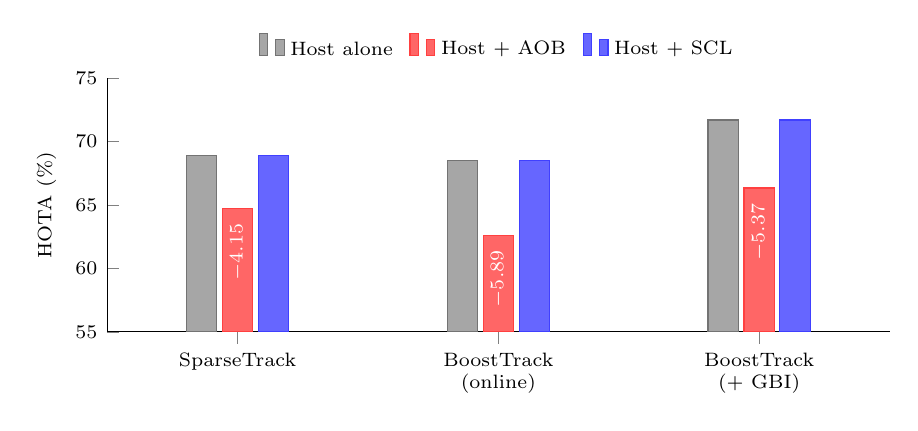
\begin{tikzpicture}
\begin{axis}[
  ybar,
  /pgf/bar width=11pt,
  width=0.95\columnwidth,
  height=4.8cm,
  ymin=55, ymax=75,
  xmin=0.5, xmax=3.5,
  xtick={1,2,3},
  xticklabels={SparseTrack, {BoostTrack\\(online)}, {BoostTrack\\(+ GBI)}},
  xticklabel style={align=center},
  ylabel={HOTA (\%)},
  axis x line*=bottom,
  axis y line*=left,
  tick label style={font=\scriptsize},
  label style={font=\scriptsize},
  legend style={at={(0.5,1.03)}, anchor=south, legend columns=3,
    font=\scriptsize, draw=none, /tikz/every even column/.append style={column sep=4pt}},
  legend cell align=left,
]
\addplot[fill=black!35, draw=black!55] coordinates {(1,68.88) (2,68.49) (3,71.72)};
\addplot[fill=red!60, draw=red!75] coordinates {(1,64.72) (2,62.61) (3,66.35)};
\addplot[fill=blue!60, draw=blue!75] coordinates {(1,68.93) (2,68.49) (3,71.72)};
\legend{Host alone, Host + \aob{}, Host + \scl{}}
\node[rotate=90, anchor=east, font=\scriptsize, text=white] at (axis cs:1,64.3) {$-4.15$};
\node[rotate=90, anchor=east, font=\scriptsize, text=white] at (axis cs:2,62.2) {$-5.89$};
\node[rotate=90, anchor=east, font=\scriptsize, text=white] at (axis cs:3,65.9) {$-5.37$};
\end{axis}
\end{tikzpicture}

\caption{HOTA on MOT17 val-half of three strong published trackers alone, with
\aob{}, and with \scl{}. The labels give the change caused by \aob{}.}
\label{fig:prior}
\end{figure}

\subsection{Design steps}\label{sec:steps}
Each step from \aob{} to \scl{} was introduced to remove one diagnosed cause
and was compared with the step before it on development data
(Table~\ref{tab:ablation}). Emulating \aob{} inside the new framework reduced
ByteTrack at floor 0.1 from 67.70 to 56.41 HOTA and OC-SORT from 66.44 to
45.72. The regime gate, which adds the regime estimate, the self-limiting
clean regime, and the crowd-safe duplicate rule, restored SparseTrack from
64.72 to 68.93 and BoostTrack from 62.61 to 68.37. Estimating the regime from
the whole stream removed regime changes in the middle of a stream and raised
ByteTrack from 67.561 to 67.702 and OC-SORT from 65.697 to 66.071. The
continuation rescue added 0.2 to 0.4 points for OC-SORT. The background check
completed \scl{}: it returned ByteTrack and BoostTrack to output identical to
the host and raised OC-SORT to 67.04 and 66.91 at the two floors. Four
variants were rejected on evidence, because they lowered HOTA, added false
positives, or let false tracks through on a noisy stream.

\begin{table*}[t]
\caption{Design steps from always-on banding (\aob{}) to \scl{} on development
data (HOTA, \%), and variants that were tested and rejected. The floor of
ByteTrack and OC-SORT is given in parentheses.}
\label{tab:ablation}
\centering\footnotesize
\setlength{\tabcolsep}{4pt}
\begin{tabular}{@{}>{\raggedright\arraybackslash}p{30mm}>{\raggedright\arraybackslash}p{44mm}>{\raggedright\arraybackslash}p{78mm}@{}}
\toprule
Step & Change & Effect\\
\midrule
\aob{} emulated & always-noisy bands, overlap deduplication, rank remap & ByteTrack (0.1) 56.41 vs host 67.70; OC-SORT (0.1) 45.72 vs 66.44\\
+ regime gate & regime statistic, host-anchored clean regime, crowd-safe duplicates & SparseTrack 64.72 to 68.93 (host 68.88); BoostTrack 62.61 to 68.37 (host 68.49)\\
+ whole-stream regime & regime from all past frames & ByteTrack (0.1) 67.561 to 67.702; OC-SORT (0.1) 65.697 to 66.071\\
+ continuation rescue & foreground track-consistent rescue & OC-SORT (0.01) 66.405 to 66.619; OC-SORT (0.1) 66.071 to 66.469\\
+ background check = \scl{} & no background mode gives no evidence against the host & ByteTrack/BoostTrack (0.1) identical to host; OC-SORT 67.041 (0.01), 66.907 (0.1)\\
\midrule
\multicolumn{2}{@{}l}{\textit{Rejected variant}} & \textit{Evidence}\\
\multicolumn{2}{@{}l}{no candidates at frame 1} & $-0.3$ to $-0.5$ HOTA on every MOT17 host\\
\multicolumn{2}{@{}l}{rescue below a two-stage host's low stage} & FP $+700$ to $+1000$, $-0.4$ to $-0.5$ HOTA\\
\multicolumn{2}{@{}l}{rank-remapped scores in clean frames} & ByteTrack $-0.2$ / $-1.6$ HOTA\\
\multicolumn{2}{@{}l}{host-clipped noisy primary band} & KITTI YOLOv8n ByteTrack $+1.4$ HOTA but uncontrolled false tracks on a noisy aerial stream (26.9 vs 14.9 boxes/frame)\\
\bottomrule
\end{tabular}
\end{table*}


\subsection{Freeze and tests}\label{sec:freeze}
The final configuration was frozen before any external evaluation. It was
recorded in a version-control tag and protected by a lock file that holds
cryptographic hashes of the layer, its configuration, and the evaluation
runners. Every later run verified the lock before running. Sixty-one automated
tests check that the layer uses no future data, that its state resets between
sequences, that clean streams pass through unchanged, that the output does not
depend on detector, tracker, or sequence names, that affine score transforms
leave the bands unchanged where designed, and that the lock is intact.

\section{Experimental Setup}\label{sec:setup}

\subsection{Hosts and baselines}\label{sec:hosts}
Nine published trackers serve as hosts: ByteTrack \cite{zhang2022bytetrack},
BoT-SORT \cite{aharon2022botsort}, OC-SORT \cite{cao2023ocsort}, SparseTrack
\cite{liu2025sparsetrack}, BoostTrack \cite{stanojevic2024boosttrack},
PD-SORT \cite{wang2025pdsort}, Hybrid-SORT \cite{yang2024hybridsort},
C-TWiX \cite{miah2025twix}, and TrackTrack \cite{shim2025tracktrack}. A tenth,
TOPICTrack \cite{cao2025topictrack}, was run but did not meet the reproduction
criterion below. Each host uses the authors' code and published configuration,
and its contract is given in Table~\ref{tab:contracts}.

In every comparison the baseline is the host alone: the published tracker run
by us with its published configuration and the same detections. The second
arm adds the frozen \scl{} and changes nothing else. Both arms run in the same
environment. Where the authors report their own numbers, these are listed
next to our reproduction of the host.

\subsection{Detectors and data}\label{sec:data}
Table~\ref{tab:data} lists the evaluation cells. On MOT17 val-half
\cite{milan2016mot16} the trackers use the published YOLOX-X detections
\cite{ge2021yolox}. The emission floor, the lowest detector score passed on,
is 0.01 or 0.1 (Table~\ref{tab:mot17}). On KITTI tracking training \cite{geiger2012kitti}, three trackers run
with two detectors that differ from the MOT17 detector: YOLOv8n
\cite{jocher2023yolov8} and RT-DETR-L \cite{zhao2024rtdetr}. To isolate the
calibration problem, the published MOT17 detections were also transformed
before the tracker by four monotone maps: cubing ($s^3$), halving ($0.5\,s$),
and logit temperatures $T=2$ and $T=0.5$, $\sigma(z/T)$. The trackers kept
their published thresholds. The external systems use the authors' released
detections on MOT17 val-half, KITTI MOTS val, and DanceTrack val
\cite{sun2022dancetrack}.

\begin{table*}[t]
\caption{Evaluation cells and their role. Development cells were visible while
the layer was designed; predeclared and post-freeze cells were run once with
the frozen policy.}
\label{tab:data}
\centering\footnotesize
\setlength{\tabcolsep}{4pt}
\begin{tabular}{@{}>{\raggedright\arraybackslash}p{36mm}>{\raggedright\arraybackslash}p{32mm}>{\raggedright\arraybackslash}p{50mm}>{\raggedright\arraybackslash}p{30mm}@{}}
\toprule
Data & Detector & Trackers & Role\\
\midrule
MOT17 val-half (7 sequences) & published YOLOX-X detections & ByteTrack (2 settings), OC-SORT, BoostTrack, SparseTrack & development\\
KITTI tracking training (21 sequences) & YOLOv8n, RT-DETR-L & ByteTrack, BoT-SORT, OC-SORT & development (detector transfer)\\
MOT17 val-half, score transforms & published YOLOX-X, transformed scores & ByteTrack (2 settings), OC-SORT, BoostTrack & development (robustness)\\
MOT17 val-half & released PD-SORT / Hybrid-SORT detections & PD-SORT, Hybrid-SORT & predeclared external\\
MOT17 val-half, KITTI MOTS val (9 sequences), DanceTrack val (25 sequences) & authors' released detections & C-TWiX, TrackTrack (DanceTrack), TOPICTrack (MOT17) & post-freeze external\\
\bottomrule
\end{tabular}
\end{table*}


\subsection{Evaluation roles}\label{sec:roles}
Every cell has one of three roles (Table~\ref{tab:data}). Development cells
were visible while the layer was designed: MOT17 with four trackers, KITTI
with three trackers and two detectors, and the score transforms. The
predeclared external systems, PD-SORT and Hybrid-SORT, were selected and
declared before they were run, and they were run once. The post-freeze
external systems, C-TWiX, TrackTrack, and TOPICTrack, were selected under a
protocol registered before any run. The protocol fixed the host contracts, the
reproduction criteria, and predictions of the layer's effect. A system entered
the analysis only if its host reproduced the authors' number: EXACT within
0.2 HOTA, or CLOSE within 1.0 HOTA with a documented, untuned cause.

\subsection{Metrics and statistics}\label{sec:metrics}
Results are reported as HOTA \cite{luiten2021hota}, MOTA
\cite{bernardin2008clear}, and IDF1 \cite{ristani2016idf1}. They are computed
with the TrackEval library (commit 12c8791) and the official ground truth of
each benchmark, following MOTChallenge practice
\cite{dendorfer2021motchallenge}. On KITTI tracking, HOTA is the official
value averaged over cars and pedestrians.

All comparisons are paired. Differences are pooled over sequences, and their
95\% intervals come from a percentile bootstrap over sequences
\cite{efron1993bootstrap} with 10,000 resamples and seed 42. A difference is
called significant when its interval excludes zero. As a distribution-free
complement, per-sequence wins, ties ($|\Delta\mathrm{HOTA}|<0.01$), and losses
are also counted.

\subsection{Latency measurement}\label{sec:latency-setup}
Latency was measured after the freeze on one cloud machine with a 4-vCPU
Intel Xeon processor at 2.10 GHz, 15 GB of memory, and no GPU. A live YOLOv8n
detector (32-bit floats, 736 pixels, batch 1) feeds ByteTrack on three KITTI
tracking sequences (0001, 0009, and 0019). Both arms run on the same frames
back to back, and the first ten frames of each sequence are excluded, which
leaves 2,279 timed frames per arm. The time of the layer includes the motion
cue, the per-frame step, and the storage of the tracker output.

\section{Results}\label{sec:results}

Figure~\ref{fig:forest} summarizes the HOTA difference between each host with
\scl{} and the host alone for every evaluated cell. The following
subsections give the baseline comparison for each part of the evaluation.

\begin{figure}[t]
\centering
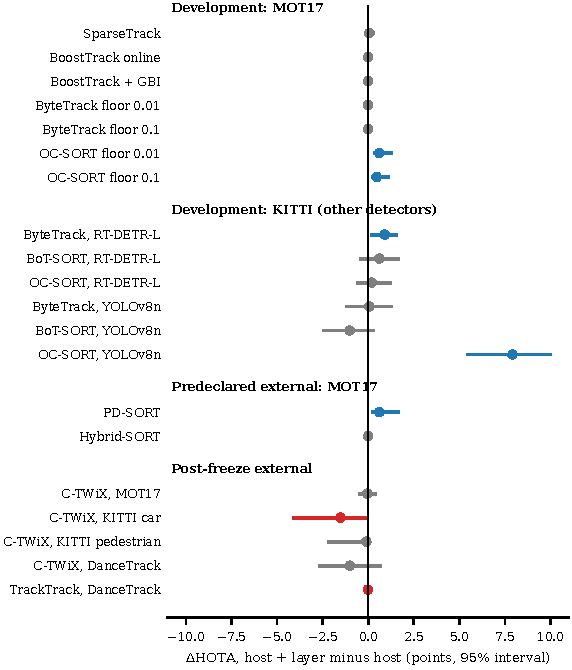
\includegraphics[width=\columnwidth]{figures/fig3_forest_col.pdf}
\caption{Difference in HOTA (host with \scl{} minus host alone) with
95\% paired-bootstrap interval for every evaluated cell. Blue: above zero;
red: below zero; gray: includes zero or identical output.}
\label{fig:forest}
\end{figure}

\subsection{Tracker transfer}\label{sec:tracker}
Table~\ref{tab:mot17} compares the development trackers with their hosts on
MOT17. The two-stage trackers with well-matched detections stayed at the
accuracy of their hosts. BoostTrack, online and with interpolation, and
ByteTrack at floor 0.1 produced identical output. ByteTrack at floor 0.01
changed by $-0.014$ HOTA and SparseTrack by $+0.055$. This is the
self-limiting behavior of the clean regime (Sect.~\ref{sec:regimes}), which
the prior design did not have (Table~\ref{tab:prior}).

The single-stage OC-SORT improved at both emission floors. Its HOTA rose by
0.61 points ($[+0.36,+1.24]$) at floor 0.01 and by 0.46 points
($[+0.27,+1.09]$) at floor 0.1, and its MOTA by 1.27 and 1.26 points. HOTA
was higher on 7 of 7 sequences in both settings (Fig.~\ref{fig:perseq}). The
gain comes from the continuation rescue. OC-SORT discards every detection
below its single threshold, and the layer passes it the foreground candidates
that continue a track that would otherwise stay unmatched.

\begin{table}[t]
\caption{Baseline comparison of the development trackers on MOT17 val-half
(published YOLOX-X detections). Paper: number reported by the tracker's
authors. Host: published tracker alone (our reproduction). $\Delta$: host with
\scl{} minus host, with 95\% paired-bootstrap interval (10,000
resamples, seed 42); bold intervals exclude zero. The floor is the lowest
detector score emitted.}
\label{tab:mot17}
\centering\footnotesize
\setlength{\tabcolsep}{4pt}
\begin{tabular}{@{}lrrl@{}}
\toprule
Metric & Paper & Host & $\Delta$ [95\% CI]\\
\midrule
\multicolumn{4}{@{}l}{\textit{SparseTrack} \cite{liu2025sparsetrack}}\\
\quad HOTA & 69.2 & 68.88 & $+0.06$ [$-0.01$, $+0.25$]\\
\quad MOTA & 76.8 & 77.85 & $+0.08$ [$-0.03$, $+0.30$]\\
\quad IDF1 & 81.4 & 81.97 & $+0.16$ [$-0.02$, $+0.70$]\\
\multicolumn{4}{@{}l}{\textit{BoostTrack, online} \cite{stanojevic2024boosttrack}}\\
\quad HOTA & 68.37 & 68.49 & 0 (identical)\\
\quad MOTA & 75.56 & 75.50 & 0 (identical)\\
\quad IDF1 & 81.35 & 81.41 & 0 (identical)\\
\multicolumn{4}{@{}l}{\textit{BoostTrack, + GBI} \cite{stanojevic2024boosttrack}}\\
\quad HOTA & 71.33 & 71.72 & 0 (identical)\\
\quad MOTA & 80.55 & 81.03 & 0 (identical)\\
\quad IDF1 & 83.84 & 84.16 & 0 (identical)\\
\multicolumn{4}{@{}l}{\textit{ByteTrack, floor 0.01} \cite{zhang2022bytetrack}}\\
\quad HOTA & -- & 67.70 & $-0.014$ [$-0.058$, $+0.009$]\\
\quad MOTA & 76.6 & 77.60 & $+0.06$ [$-0.15$, $+0.34$]\\
\quad IDF1 & 79.3 & 79.47 & $-0.031$ [$-0.135$, $+0.035$]\\
\multicolumn{4}{@{}l}{\textit{ByteTrack, floor 0.1} \cite{zhang2022bytetrack}}\\
\quad HOTA & -- & 67.70 & 0 (identical)\\
\quad MOTA & 76.6 & 77.60 & 0 (identical)\\
\quad IDF1 & 79.3 & 79.47 & 0 (identical)\\
\multicolumn{4}{@{}l}{\textit{OC-SORT, floor 0.01} \cite{cao2023ocsort}}\\
\quad HOTA & 66.5 & 66.43 & {\boldmath $+0.61$ [$+0.36$, $+1.24$]}\\
\quad MOTA & 74.9 & 74.67 & {\boldmath $+1.27$ [$+0.17$, $+3.01$]}\\
\quad IDF1 & 77.7 & 78.05 & $+0.66$ [$-0.25$, $+1.60$]\\
\multicolumn{4}{@{}l}{\textit{OC-SORT, floor 0.1} \cite{cao2023ocsort}}\\
\quad HOTA & 66.5 & 66.44 & {\boldmath $+0.46$ [$+0.27$, $+1.09$]}\\
\quad MOTA & 74.9 & 74.67 & {\boldmath $+1.26$ [$+0.37$, $+3.34$]}\\
\quad IDF1 & 77.7 & 78.05 & {\boldmath $+0.287$ [$+0.003$, $+0.838$]}\\
\bottomrule
\end{tabular}
\end{table}


\begin{figure}[t]
\centering
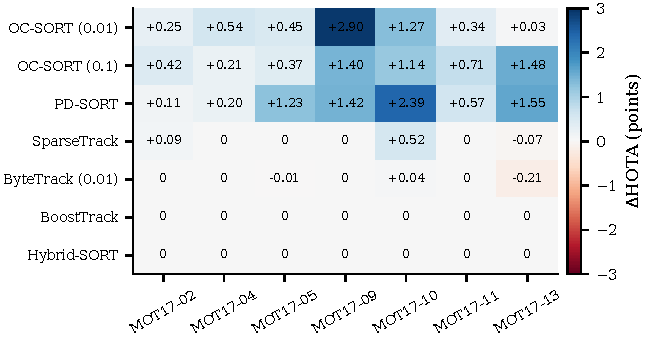
\includegraphics[width=\columnwidth]{figures/fig4_per_sequence.pdf}
\caption{Per-sequence HOTA differences (host with \scl{} minus host
alone) on MOT17 val-half for the development and predeclared trackers.}
\label{fig:perseq}
\end{figure}

\subsection{Detector change}\label{sec:detector}
Table~\ref{tab:kitti} reports three trackers with two detectors on KITTI. With
the noisy RT-DETR-L stream, the two-stage trackers gained in MOTA and IDF1.
ByteTrack gained 5.98 MOTA points ($[+1.16,+9.94]$), 3.87 IDF1 points, and
0.91 HOTA points ($[+0.22,+1.55]$). BoT-SORT gained 7.86 MOTA points
($[+2.21,+13.44]$) and 3.10 IDF1 points. With YOLOv8n, the single-stage
OC-SORT gained 7.91 HOTA points ($[+5.47,+9.98]$), 9.40 MOTA points, and 9.60
IDF1 points.

\begin{table}[t]
\caption{Baseline comparison under a detector change on KITTI tracking
training (official HOTA, car and pedestrian averaged). Host: published
tracker alone with the same detections. $\Delta$: host with \scl{}
minus host, with 95\% paired-bootstrap interval; bold intervals exclude zero.
BoT-SORT excludes one sequence on which the unmodified tracker fails
numerically.}
\label{tab:kitti}
\centering\footnotesize
\setlength{\tabcolsep}{4pt}
\begin{tabular}{@{}lrl@{}}
\toprule
Metric & Host & $\Delta$ [95\% CI]\\
\midrule
\multicolumn{3}{@{}l}{\textit{ByteTrack} \cite{zhang2022bytetrack}\textit{, RT-DETR-L}}\\
\quad HOTA & 50.73 & {\boldmath $+0.91$ [$+0.22$, $+1.55$]}\\
\quad MOTA & 47.27 & {\boldmath $+5.98$ [$+1.16$, $+9.94$]}\\
\quad IDF1 & 64.98 & {\boldmath $+3.87$ [$+1.67$, $+5.06$]}\\
\multicolumn{3}{@{}l}{\textit{BoT-SORT} \cite{aharon2022botsort}\textit{, RT-DETR-L}}\\
\quad HOTA & 53.91 & $+0.61$ [$-0.39$, $+1.61$]\\
\quad MOTA & 48.25 & {\boldmath $+7.86$ [$+2.21$, $+13.44$]}\\
\quad IDF1 & 67.74 & {\boldmath $+3.10$ [$+1.00$, $+4.57$]}\\
\multicolumn{3}{@{}l}{\textit{OC-SORT} \cite{cao2023ocsort}\textit{, RT-DETR-L}}\\
\quad HOTA & 52.64 & $+0.19$ [$-0.57$, $+1.19$]\\
\quad MOTA & 57.59 & $-0.57$ [$-4.36$, $+1.40$]\\
\quad IDF1 & 69.87 & $+0.04$ [$-1.31$, $+1.78$]\\
\multicolumn{3}{@{}l}{\textit{ByteTrack} \cite{zhang2022bytetrack}\textit{, YOLOv8n}}\\
\quad HOTA & 45.31 & $+0.06$ [$-1.19$, $+1.24$]\\
\quad MOTA & 46.54 & $-1.87$ [$-6.25$, $+0.03$]\\
\quad IDF1 & 60.92 & $+1.49$ [$-0.36$, $+3.27$]\\
\multicolumn{3}{@{}l}{\textit{BoT-SORT} \cite{aharon2022botsort}\textit{, YOLOv8n}}\\
\quad HOTA & 49.21 & $-1.02$ [$-2.43$, $+0.25$]\\
\quad MOTA & 49.89 & {\boldmath $-2.43$ [$-7.43$, $-0.14$]}\\
\quad IDF1 & 64.41 & $+0.35$ [$-2.10$, $+2.27$]\\
\multicolumn{3}{@{}l}{\textit{OC-SORT} \cite{cao2023ocsort}\textit{, YOLOv8n}}\\
\quad HOTA & 36.27 & {\boldmath $+7.91$ [$+5.47$, $+9.98$]}\\
\quad MOTA & 33.99 & {\boldmath $+9.40$ [$+1.10$, $+12.30$]}\\
\quad IDF1 & 50.46 & {\boldmath $+9.60$ [$+5.61$, $+12.16$]}\\
\bottomrule
\end{tabular}
\end{table}


\subsection{Detector confidence shift}\label{sec:shift}
Table~\ref{tab:shift} and Fig.~\ref{fig:shift} give the trackers under the
four score transforms. Halving the scores drove ByteTrack (official setting)
and OC-SORT to 0 HOTA, because no detection reached their thresholds. With the
layer they reached 66.17 and 66.72. Cubing reduced them to 60.92 and 58.34,
and the layer restored them to 65.81 and 66.60. BoostTrack rose from 61.33 to
64.84 under cubing. With temperature $T=2$, the layer raised ByteTrack and
OC-SORT by 1.11 and 1.24 points. The library setting of ByteTrack, whose low
thresholds already admit the shifted scores, stayed within 0.14 points in all
four transforms. Over the 14 conditions, the layer raised HOTA significantly
in 7 and lowered it significantly in none.

\begin{table}[t]
\caption{Baseline comparison under detector confidence shift on MOT17 val-half
(HOTA). The detector scores are transformed before the tracker, whose
published thresholds stay fixed; $T$ is a logit temperature, $\sigma(z/T)$.
Host: published tracker alone. $\Delta$: with \scl{} minus host,
with 95\% paired-bootstrap interval (10,000 resamples, seed 42). Bold
intervals exclude zero. Emission floor 0.01 (BoostTrack 0.1).}
\label{tab:shift}
\centering\footnotesize
\setlength{\tabcolsep}{4pt}
\begin{tabular}{@{}lrrl@{}}
\toprule
Transform & Host & + \scl{} & $\Delta$HOTA\\
\midrule
\multicolumn{4}{@{}l}{\textit{ByteTrack, official setting} \cite{zhang2022bytetrack}}\\
\quad $s^3$ & 60.92 & 65.81 & {\boldmath $+4.89$ [$+2.60$, $+13.69$]}\\
\quad $0.5\,s$ & 0.00 & 66.17 & {\boldmath $+66.17$ [$+49.32$, $+75.40$]}\\
\quad $T=2$ & 65.84 & 66.95 & {\boldmath $+1.11$ [$+0.35$, $+3.87$]}\\
\quad $T=0.5$ & 67.30 & 67.29 & $-0.009$ [$-0.051$, $+0.005$]\\
\multicolumn{4}{@{}l}{\textit{ByteTrack, library setting} \cite{zhang2022bytetrack}}\\
\quad $s^3$ & 66.31 & 66.31 & $-0.006$ [$-0.384$, $+0.383$]\\
\quad $0.5\,s$ & 66.61 & 66.48 & $-0.14$ [$-0.66$, $+0.14$]\\
\quad $T=2$ & 63.97 & 63.97 & 0 (identical)\\
\quad $T=0.5$ & 66.53 & 66.52 & $-0.006$ [$-0.029$, $+0.001$]\\
\multicolumn{4}{@{}l}{\textit{OC-SORT} \cite{cao2023ocsort}}\\
\quad $s^3$ & 58.34 & 66.60 & {\boldmath $+8.26$ [$+5.86$, $+16.81$]}\\
\quad $0.5\,s$ & 0.00 & 66.72 & {\boldmath $+66.72$ [$+50.32$, $+75.56$]}\\
\quad $T=2$ & 65.99 & 67.22 & {\boldmath $+1.24$ [$+0.52$, $+3.42$]}\\
\quad $T=0.5$ & 66.61 & 67.06 & $+0.45$ [$-0.01$, $+0.97$]\\
\multicolumn{4}{@{}l}{\textit{BoostTrack, online} \cite{stanojevic2024boosttrack}}\\
\quad $s^3$ & 61.33 & 64.84 & {\boldmath $+3.51$ [$+0.85$, $+13.28$]}\\
\quad $T=2$ & 67.59 & 67.59 & 0 (identical)\\
\bottomrule
\end{tabular}
\end{table}


\begin{figure*}[t]
\centering
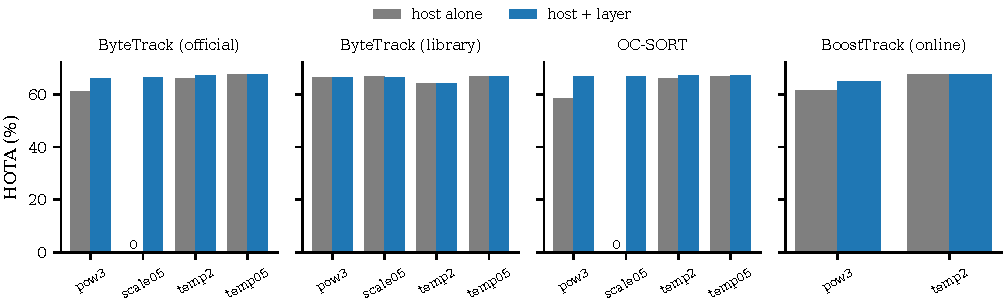
\includegraphics[width=0.9\textwidth]{figures/fig5_calibration_shift.pdf}
\caption{Detector confidence shift on MOT17 val-half: HOTA of each published
tracker with its published thresholds, alone and with \scl{}, after
four monotone transforms of the detector scores (pow3: $s^3$; scale05:
$0.5\,s$; temp2 and temp05: $T=2$ and $T=0.5$).}
\label{fig:shift}
\end{figure*}

\subsection{External systems}\label{sec:external}
Table~\ref{tab:external} gives every external system. PD-SORT
\cite{wang2025pdsort} was reproduced identically to the authors' released
output. With \scl{}, its HOTA rose by 0.61 points ($[+0.27,+1.65]$), its
MOTA by 1.13 points ($[+0.27,+3.03]$), and its IDF1 by 0.82 points
($[+0.43,+1.94]$), with higher HOTA on 7 of 7 sequences
(Fig.~\ref{fig:perseq}). False negatives fell by 1,291, and false positives
rose by 681. PD-SORT is a single-stage tracker, and its gain follows the same
mechanism as for OC-SORT; unlike OC-SORT, it was not seen during design.
Hybrid-SORT \cite{yang2024hybridsort}, a two-stage tracker, produced identical
output, as predicted before the run.

After the freeze, C-TWiX \cite{miah2025twix} was reproduced on three datasets
and TrackTrack \cite{shim2025tracktrack} on DanceTrack, all within the
reproduction criterion. Their results are listed in Table~\ref{tab:external}. On
DanceTrack, the output of TrackTrack with \scl{} was tied with the host on
21 of 25 sequences.

\begin{table*}[t]
\caption{Baseline comparison on the external systems, each evaluated once with
the frozen \scl{}. Reference / reproduced: the authors' HOTA and the HOTA of
the host alone in our runs. Reproduction class against the authors' number
(EXACT: $|\Delta\mathrm{HOTA}|\le0.2$; CLOSE: $\le1.0$ with a documented,
untuned cause). $\Delta$: host with \scl{} minus host, with 95\%
paired-bootstrap interval; bold intervals exclude zero. TOPICTrack failed
reproduction and is excluded from the analysis.}
\label{tab:external}
\centering\footnotesize
\setlength{\tabcolsep}{4pt}
\begin{tabular}{@{}lccccc@{}}
\toprule
System & Reference / & Class & $\Delta$HOTA & $\Delta$MOTA & $\Delta$IDF1\\
(data) & reproduced & & & & \\
\midrule
\multicolumn{6}{@{}l}{\textit{Predeclared before the runs}}\\
\twol{PD-SORT \cite{wang2025pdsort}}{MOT17 val-half} & 68.01 / 68.01 & \twol{EXACT}{(released output)} & \cib{+0.61}{+0.27}{+1.65} & \cib{+1.13}{+0.27}{+3.03} & \cib{+0.82}{+0.43}{+1.94}\\[6pt]
\twol{Hybrid-SORT \cite{yang2024hybridsort}}{MOT17 val-half} & 67.1 / 66.70 & CLOSE & 0 (identical) & 0 (identical) & 0 (identical)\\[2pt]
\multicolumn{6}{@{}l}{\textit{Post-freeze, protocol registered before the runs}}\\
\twol{C-TWiX \cite{miah2025twix}}{MOT17 val-half} & 77.8 / 77.55 & CLOSE & \ci{-0.05}{-0.46}{+0.40} & \ci{+0.24}{-0.58}{+1.12} & \ci{+0.18}{-0.47}{+1.14}\\[6pt]
\twol{C-TWiX (car)}{KITTI MOTS val} & 89.3 / 89.27 & EXACT & \cib{-1.52}{-4.05}{-0.13} & \cib{-2.11}{-5.89}{-0.17} & \cib{-1.21}{-3.32}{-0.10}\\[6pt]
\twol{C-TWiX (pedestrian)}{KITTI MOTS val} & 71.4 / 70.77 & CLOSE & \ci{-0.10}{-2.16}{+0.03} & \ci{-0.31}{-4.86}{+0.10} & \ci{-0.01}{-1.90}{+0.08}\\[6pt]
\twol{C-TWiX}{DanceTrack val} & 60.4 / 59.62 & CLOSE & \ci{-1.00}{-2.62}{+0.65} & \ci{+0.13}{-0.39}{+0.47} & \ci{-1.55}{-3.76}{+0.52}\\[6pt]
\twol{TOPICTrack \cite{cao2025topictrack}}{MOT17 val-half} & 69.6 / 67.54 & FAILED & \multicolumn{3}{c}{not analyzed}\\[2pt]
\twol{TrackTrack \cite{shim2025tracktrack}}{DanceTrack val} & 63.3 / 62.96 & CLOSE & \cib{-0.013}{-0.032}{-0.001} & \cib{-0.073}{-0.208}{-0.004} & \ci{+0.009}{-0.001}{+0.028}\\
\bottomrule
\end{tabular}
\end{table*}


\subsection{Latency}\label{sec:latency}
Table~\ref{tab:runtime} and Fig.~\ref{fig:runtime} compare the per-frame time
of the host pipeline with and without \scl{}. \scl{} took 2.95 ms per
frame on average and 4.39 ms at the 95th percentile, including the
phase-correlation motion cue. The end-to-end time rose from 57.85 to 60.44 ms
per frame, by 4.5\%. The tracker became faster, from 2.04 to 1.43 ms per
frame, because it received fewer candidates. The detector takes most of each
frame, about 42 ms, so the layer adds only a small part of the total latency.

\begin{table}[t]
\caption{Baseline comparison of the per-frame time on a 4-vCPU Intel Xeon
(2.10 GHz, no GPU) with a live YOLOv8n detector (736 pixels) and ByteTrack on
three KITTI sequences (2,279 timed frames per arm). Host alone: the same
pipeline without \scl{}. Mean / 95th percentile in milliseconds.}
\label{tab:runtime}
\centering\footnotesize
\setlength{\tabcolsep}{4pt}
\begin{tabular}{@{}lcc@{}}
\toprule
Stage & Host alone & Host + \scl{}\\
\midrule
Frame decode & 13.88 / 16.21 & 13.88 / 16.51\\
Detector (YOLOv8n, 736 px) & 41.91 / 58.41 & 42.17 / 59.43\\
\scl{} & -- & 2.95 / 4.39\\
Tracker (ByteTrack) & 2.04 / 3.57 & 1.43 / 2.64\\
End to end & 57.85 / 76.35 & 60.44 / 80.78\\
\bottomrule
\end{tabular}
\end{table}


\begin{figure}[t]
\centering
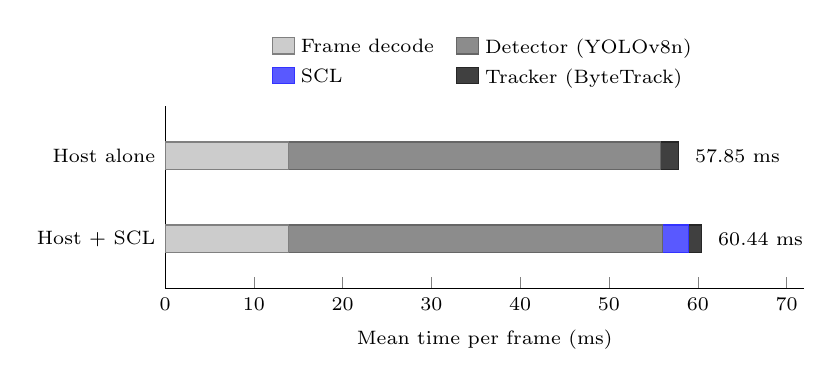
\begin{tikzpicture}
\begin{axis}[
  xbar stacked,
  /pgf/bar width=10pt,
  width=0.8\columnwidth,
  height=3.9cm,
  xmin=0, xmax=72,
  clip=false,
  ymin=-0.6, ymax=1.6,
  ytick={0,1},
  yticklabels={Host + \scl{}, Host alone},
  xlabel={Mean time per frame (ms)},
  axis x line*=bottom,
  axis y line*=left,
  tick label style={font=\scriptsize},
  label style={font=\scriptsize},
  legend style={at={(0.5,1.04)}, anchor=south, legend columns=2,
    font=\scriptsize, draw=none, /tikz/every even column/.append style={column sep=6pt}},
  legend cell align=left,
]
\addplot[fill=black!20, draw=black!50] coordinates {(13.88,1) (13.88,0)};
\addplot[fill=black!45, draw=black!60] coordinates {(41.91,1) (42.17,0)};
\addplot[fill=blue!65, draw=blue!80] coordinates {(0,1) (2.95,0)};
\addplot[fill=black!75, draw=black!85] coordinates {(2.04,1) (1.43,0)};
\legend{Frame decode, Detector (YOLOv8n), \scl{}, Tracker (ByteTrack)}
\node[anchor=west, font=\scriptsize] at (axis cs:58.6,1) {57.85 ms};
\node[anchor=west, font=\scriptsize] at (axis cs:61.2,0) {60.44 ms};
\end{axis}
\end{tikzpicture}

\caption{Mean per-frame time by stage for the host pipeline alone and with
\scl{} (4-vCPU Intel Xeon, no GPU). The labels give the measured
end-to-end time.}
\label{fig:runtime}
\end{figure}

\section{Discussion}\label{sec:discussion}

\emph{When the layer acts.} The direction of the effect follows two
properties of the pipeline rather than the dataset: whether the tracker has a
continuation stage, and whether the detector's score distribution matches the
tracker's thresholds. The regime estimate makes this visible. On the C-TWiX
streams after the freeze, 99.7\% of the MOT17 frames and 99.9\% of the
DanceTrack frames were classified clean, and the largest noisy share was 2.8\%
of the frames, on KITTI. When the stream fits the tracker, the layer stays out
of the way.

\emph{Self-limiting by design.} In the clean regime the layer keeps the
tracker's thresholds and scores, so a tracker with a low-score stage and
well-matched detections receives its native input. This is the main
difference from the prior design \aob{}, which lowered the HOTA of the same strong
trackers by 4.15 to 5.89 points (Table~\ref{tab:prior}). The layer therefore does not
need to know in advance whether a tracker needs help; it reads the answer from
the score stream.

\emph{A continuation stage for single-stage trackers.} Single-stage trackers
drop every detection below one threshold, so a track can be lost when its
object scores low for a few frames. The continuation rescue considers only
candidates that overlap a track of the previous frame that no usable candidate
covers, so it targets exactly these gaps. OC-SORT and the external PD-SORT
gained HOTA on 7 of 7 MOT17 sequences through this stage.

\emph{Detector replacement.} When a detector is replaced or its confidence
scale shifts, the fixed thresholds of a tracker stop matching the scores. The
layer re-anchors them from the score stream without labels. Under halved
scores it restored two trackers from 0 to about 66 HOTA, and with a different
detector it raised the MOTA of two two-stage trackers by 6.0 and 7.9 points.
This is the situation the layer was built for: a detector that is swapped,
retrained, or quantized while the tracker stays fixed.

\emph{Real-time deployment.} The layer needs no training, no GPU, and no
access to the detector's internals, and it needs only four contract values
from the tracker's configuration. At run time it reads the candidate list, one
small grayscale image for the motion cue, and the tracks of the previous
frame. On a four-core CPU it takes 2.95 ms per frame, adds 4.5\% to the end-to-end time, and makes the tracker
itself faster. \scl{} therefore adds very little latency and is
suitable for real-time use. New trackers are added through their published
contract values and an adapter, without changes to the policy.

\section{Conclusion}\label{sec:conclusion}

This paper presented \scl{}, a training-free control layer that calibrates itself
from a detector's score stream and adapts a frozen tracker through a declared
host contract. The layer splits the logits of recent frames with nested Otsu
thresholds, estimates whether the stream is clean or noisy, keeps the
tracker's operating point on clean streams, and selects candidates, remaps
scores, and sets thresholds on noisy streams. A continuation rescue gives
single-stage trackers the stage they lack.

\scl{} was developed from always-on banding (\aob{}), an earlier design that
intervened in every frame, and each step was compared with that baseline. One frozen configuration was then evaluated on
nine published trackers, four detection sources, and three datasets with
development, predeclared, and post-freeze roles. It raised the HOTA of
OC-SORT and of the predeclared external PD-SORT by 0.61 points, restored
trackers whose thresholds no longer matched a shifted confidence scale, raised
the MOTA of two-stage trackers with a noisy detector by 6.0 and 7.9 points,
and left well-matched two-stage pipelines at their own accuracy. It costs
2.95 ms per frame on a CPU. These results support placing a self-calibrating
layer between the detector and the tracker in pipelines where the detector
changes while the tracker stays fixed.


\backmatter

\section*{Declarations}

\noindent\textbf{Funding.} This research received no external funding.

\noindent\textbf{Conflict of interest.} The authors declare no competing interests.

\noindent\textbf{Ethics approval and consent to participate.} This computational study uses public benchmark data and does not involve human participants or animals.

\noindent\textbf{Consent for publication.} Not applicable.

\noindent\textbf{Data availability.} All datasets used (MOT17, KITTI tracking, DanceTrack) are publicly available from their providers. Tracker outputs, bootstrap records, and the frozen configuration are available from the corresponding author on reasonable request.

\noindent\textbf{Code availability.} The implementation of \scl{} and the evaluation scripts are available from the corresponding author on reasonable request.

\noindent\textbf{Author contributions.} Ahmed Gouda Ismail: Conceptualization, Methodology, Software, Investigation, Formal analysis, Visualization, Writing~--~original draft. Mohamed S. Mohamed and Tarek Ahmed Mahmoud: Supervision, Methodology, Writing~--~review \& editing. All authors read and approved the final manuscript.

\noindent\textbf{Acknowledgements.} The authors thank the authors of the evaluated trackers for releasing their code, weights, and detections, and the maintainers of MOT17, KITTI, DanceTrack, and TrackEval.

\noindent\textbf{AI use in manuscript preparation.} Generative AI tools were used to assist with drafting and language editing. The authors reviewed and verified all content, numerical values, and figures and take full responsibility for the manuscript.

\bibliography{references}

\end{document}
